\documentclass[11pt]{article}

\usepackage[margin=1.5in]{geometry}
\usepackage{lecnotes}
% \usepackage{mpass}
% \lstset{style=verb,language=mpass}
% logic macros, to be filled from
% lmacros-f21.tex (15-814, F21) and lmacros-f16 (15816, F16)

\newcommand{\ddd}{\raisebox{0.2em}[1.1em]{$\vdots$}}
\newcommand{\vctr}[1]{\begin{array}[c]{c}#1\end{array}}
\newcommand{\CC}{\mathcal{C}}
\newcommand{\DD}{\mathcal{D}}
\newcommand{\EE}{\mathcal{E}}
\newcommand{\FF}{\mathcal{F}}

\newcommand{\ms}[1]{\mathsf{#1}}
\newcommand{\mi}[1]{\mathit{#1}}
\newcommand{\mb}[1]{\mathbf{#1}}
\newcommand{\mt}[1]{\mathtt{#1}}
\newcommand{\ums}[1]{\underline{\ms{#1}}}
\newcommand{\oms}[1]{\overline{\ms{#1}}}
\newcommand{\mc}[1]{\mathcal{#1}}

\newcommand{\uscore}{\mbox{\tt\char`\_}}
\newcommand{\arrow}{\mathbin{\rightarrow}}

\newcommand{\semi}{\mathrel{;}}

% from stmaryrd
\newcommand{\lbb}{\llbracket}
\newcommand{\rbb}{\rrbracket}

% evaluation
\newcommand{\eval}{\ms{eval}}
\newcommand{\evalz}{\ms{eval}_{\mathbb{Z}}}
\newcommand{\evalb}{\ms{eval}_{\mathbb{B}}}

% authorization logic
\newcommand{\says}{\mathrel{\mb{says}}}
\newcommand{\aff}{\mathrel{\mb{aff}}}
\newcommand{\llet}[3]{\mb{let}\; #1 = #2\; \mb{in}\; #3}
\newcommand{\alet}[4]{\mb{let}\; \{#1\}_{#2} = #3\; \mb{in}\; #4}

% \newcommand{\rep}[1]{{}^\ulcorner\! #1{}^\urcorner}

\newcommand{\new}[1]{{\color{blue}#1}}





\newcommand{\course}{15-316: Software Foundations of Security \& Privacy}
\newcommand{\lecturer}{Matt Fredrikson}
\newcommand{\lecdate}{February 19, 2026}
\newcommand{\lecnum}{11}
\newcommand{\lectitle}{Beyond Safety Properties}
\newcommand{\courseurl}{https://15316-cmu.github.io/2026/}

\begin{document}

\maketitle

\section{Introduction}

Recall that a \emph{trace} of a program is the (potentially infinite) sequence
of states that make up its computation.  A \emph{safety property} of a trace is
defined as one whose violation can be determined from a finite prefix.  A
\emph{liveness property} is one whose violation may depend on the whole infinite
trace.  Operations such as division by zero or out-of-bounds memory access are
examples of safety properties.  We can prove safety in dynamic logic via
propositions of the form $P \arrow [\alpha]\top$.  Examples of liveness
properties would be that a server responds to a query or that a lock acquired in
a concurrent computation is eventually released.  We can prove liveness
properties in dynamic logic via propositions of the form
$P \arrow \langle \alpha\rangle Q$ (pronounced ``\emph{diamond alpha Q}'').
Recall that the formula $\langle \alpha\rangle Q$ is true if there is a way to
reach a final state such that $Q$ is true.  This implies that, among other
things, loops appearing in the computation must be proved terminating.  We have
deemphasized the diamond modality, not investigating its properties.

There are techniques for transforming liveness properties into safety
properties.  For example, we can require that a server respond within a certain
number of steps or milliseconds.  However, it may still be difficult to enforce
such transformed liveness properties, and it may be even more difficult to take
appropriate corrective action.

Today we will start analyzing an important class of security policies, called
\emph{information flow policies}, that go beyond both safety and liveness
properties in the sense that we cannot determine if they are violated by
analyzing a single program trace.

\section{Information Flow, Informally}

When you log in to your favorite banking site, you would like to be able to see
information about your own account, but you should not be able to see anyone
else's.  In other words, we don't want information to flow from other accounts
to the program serving you.  In our small imperative language we model this
using \emph{high security variables} and \emph{low security variables}.  Reading
from a high security variable and writing the value to a low security variable
would be a violation of our information flow policy.  It would be slightly more
realistic to consider reading and writing from memory, but it would be more
complex without changing the fundamental ideas we study.

As a small running example we consider the following program.
\[
  \begin{array}{ll}
    x := 1 \semi \\
    y := x + 5 \semi \\
    z := y - 1
  \end{array}
\]
We consider $x$ to be a high security variables, while $y$ and $z$ are
classified as low security.  We write this information flow policy as
\[
  x : \ms{H}, y : \ms{L}, z : \ms{L}
\]
Intuitively, the program above would not satisfy our security policy: we read
from $x$ (high security) and then write $x+5$ to $y$, which is low security.  In
fact, we can exactly recover $x$ as $y - 5$, so we gain perfect information
about a secret.

Here is a trace of this program, assuming all variables initially have value $0$.
\[
  \begin{array}{ll}
    & (x = 0, y = 0, z = 0) \\
    \Rightarrow & (x = 1, y = 0, z = 0) \\
    \Rightarrow & (x = 1, y = 6, z = 0) \\
    \Rightarrow & (x = 1, y = 6, z = 5)
  \end{array}
\]
Now consider the following alternative program shown on the right.
\[
  \begin{array}{l@{\hspace{2em}}|@{\hspace{2em}}l@{\hspace{2em}}|@{\hspace{2em}}l@{\hspace{2em}}l}
    (x = 0, y = 0, z = 0) &  x := 1 \semi & x := 1 \semi \\ 
    (x = 1, y = 0, z = 0) &  y := x + 5 \semi & y := 6 \semi \\
    (x = 1, y = 6, z = 0) &  z := y - 1 & z := 5  &     \\
    (x = 1, y = 6, z = 5) & & 
  \end{array}
\]
We see that both programs have \emph{exactly the same trace}, but the first
one violates the policy (information flows from $x$ to $y$ and then to $z$)
while no information flows at all on the right.

This shows that information flow is not a property of a single trace of a
program, but requires something more.  We'll see what in the next lecture.
Meanwhile, we'll try to intuit a program analysis that ensures adherence to an
information flow policy.  In the next lecture, we will check if it accomplishes
what a semantic definition of information flow demands.

\section{Tracking Security Levels}

We now consider ways analyze programs with the goal of proving that a given
information flow policy is respected by a program.  Because we haven't
rigorously defined what that is, the remainder of this lecture is rather
speculative.  In the next lecture we will nail it down precisely.

For now, we imagine a security policy is given by an assignment of security
levels to variables, like $\ms{H}$ for \emph{high} and $\ms{L}$ for \emph{low}.
We use $\Sigma$ as a map from variables to security levels.  We write $x : \ell$
if the variable $x$ has security level $\ell$.  Our system of inference rules
derive
\[
  \Sigma \vdash \alpha\; \ms{secure}
\]
which expresses that, given the security policy $\Sigma$, the program $\alpha$
is secure.  We name the inference rules as $\mi{name}T$, where $T$ stands for
\emph{taint} (see \autoref{sec:taint}).

\paragraph{Assignment.}  At the root of the system is that an assignment
$x := e$ is a violation of the security policy if $x : \ms{L}$ and $e : \ms{H}$.
The security level of an expression is the maximal level of the variables
occurring in it.  That is, we also define $\Sigma \vdash e : \ell$, meaning that
expression $e$ has security level $\ell$.

Variables just have the level prescribed by the policy, and constants are always
of low security.
\begin{rules}
  \infer[\ms{var}T]
  {\Sigma \vdash x : \ell}
  {\Sigma(x) = \ell}
  \hspace{3em}
  \infer[\ms{const}T]
  {\Sigma \vdash c : \ms{L}}
  {}
\end{rules}
For a binary operator, we take the maximal security level of the constituents,
where $\ms{H} > \ms{L}$.
\begin{rules}
  \infer[\ms{+}T]
  {\Sigma \vdash e_1 + e_2 : \ell}
  {\Sigma \vdash e_1 : \ell_1
    & \Sigma \vdash e_2 : \ell_2
    & \ell = \mathrm{max}(\ell_1, \ell_2)}
\end{rules}
For an assignment, there are several possible combinations.  The first: we can
always write to a high security variable, since this does not represent a flow
from high to low.  An example of this could be appending to a (secure) log file
using a low-security value.
\begin{rules}
  \infer[\mb{:=}T_1]
  {\Sigma \vdash x := e\; \ms{secure}}
  {\Sigma(x) = \ms{H}}
\end{rules}
If $x$ is of low security, then $e$ also has to be (or we fail).
\begin{rules}
  \infer[\mb{:=}T_2]
  {\Sigma \vdash x := e\; \ms{secure}}
  {\Sigma(x) = \ms{L}
    & \Sigma \vdash e : \ms{L}}
  \hspace{3em}
  \infer-[]
  {\Sigma \vdash x := e\; \ms{secure}}
  {\mbox{\textbf{no rule for}}
    & \Sigma(x) = \ms{L}
    & \Sigma \vdash e : \ms{H}}
\end{rules}

\section{A Lattice of Security Levels}

Before we go further, we generalize the security levels from just two (high and
low) to potentially multiple ones.  We imagine them being arranged in a
\emph{lattice}, where information is allowed to flow upwards but not downwards.
I think that technically we just need a \emph{join-semilattice}, although
different authors make slightly different assumptions.

Below are two examples. This first just has the high and low security levels we
have been using.  The second is one where we imagine three principals,
$\ms{p}_1$, $\ms{p}_2$, and $\ms{p}_3$, say bank account holders.  They cannot
see high security values (level $\ms{H}$) and they cannot see each other's data
since information can only flow up but not down.  The lowest level $\ms{L}$ is
``public'' (anyone can see it).
\[
  \begin{tikzpicture}
    \node (h) at (0,1) {$\ms{H}$};
    \node (l) at (0,0) {$\ms{L}$};
    \draw[thick] (h) -- (l);
  \end{tikzpicture}
  \hspace{5em}
  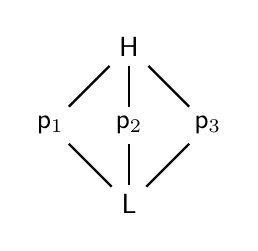
\begin{tikzpicture}
    \node (h) at (1,2) {$\ms{H}$}; 
    \node (p1) at (0,1) {$\ms{p}_1$}; 
    \draw[thick] (h) -- (p1); 
    \node (p2) at (1,1) {$\ms{p}_2$}; 
    \draw[thick] (h) -- (p2); 
    \node (p3) at (2,1) {$\ms{p}_3$}; 
    \draw[thick] (h) -- (p3); 
    \node (l) at (1,0) {$\ms{L}$}; 
    \draw[thick] (p1) -- (l); 
    \draw[thick] (p2) -- (l); 
    \draw[thick] (p3) -- (l); 
  \end{tikzpicture}
\]

A join-semilattice is defined by a partial order $\ell_1 \sqsubseteq \ell_2$
($\ell_1$ is a lower security level than $\ell_2$) and the operation of
$\ell_1 \sqcup \ell_2$ (the \emph{least upper bound} of two security levels).
We also need a least element $\bot$ which is the unit of $\sqcup$ and is below
every other level.  We will not go into details regarding all the algebraic laws
of the semilattice, but here are some from properties of the least upper bound
and the least element.
\[
  \begin{array}{l}
    \bot \sqcup \ell = \ell \sqcup \bot = \ell \\[1ex]
    \bot \sqsubseteq \ell \\[1ex]
    \ell_1 \sqsubseteq \ell_1 \sqcup \ell_2 \\
    \ell_2 \sqsubseteq \ell_1 \sqcup \ell_2 \\
    \ell_1 \sqsubseteq \ell \ \mbox{and}\ \ell_2 \sqsubseteq \ell\ \mbox{implies}\ 
    \ell_1 \sqcup \ell_2 \sqsubseteq \ell
  \end{array}
\]
We can generalize the rules so far from two levels to a lattice of security
levels.
\begin{rules}
  \infer[\ms{var}T]
  {\Sigma \vdash x : \ell}
  {\Sigma(x) = \ell}
  \hspace{2em}
  \infer[\ms{const}T]
  {\Sigma \vdash c : \bot}
  {}
  \hspace{2em}
  \infer[\mb{+}T]
  {\Sigma \vdash e_1 + e_2 : \ell}
  {\Sigma \vdash e_1 : \ell_1
    & \Sigma \vdash e_2 : \ell_2
    & \ell = \ell_1 \sqcup \ell_2}
  \\[1em]
  \infer[\mb{:=}T]
  {\Sigma \vdash x := e\; \ms{secure}}
  {\Sigma \vdash e : \ell
    & \ell \sqsubseteq \Sigma(x)}
\end{rules}
The last rule expresses succinctly that information can only flow from lower to
higher levels of security, and not in any other circumstances.

\section{Tracking Security Levels, Continued}

With assignment specified, we move on to other language constructs.

\paragraph{Sequential Composition.}  We check both subprograms independently
with respect to the same security policy $\Sigma$.
\begin{rules}
  \infer[\mb{\semi}T]
  {\Sigma \vdash \alpha \semi \beta\; \ms{secure}}
  {\Sigma \vdash \alpha\; \ms{secure}
    & \Sigma \vdash \beta\; \ms{secure}}
\end{rules}

At this point we have enough to check that one of our two example programs is
secure while the other one is not.  We use the two-element lattice with
$\ms{H} \sqsupset \ms{L}$ and the security policy
\[
  \Sigma_0 = (x : \ms{H}, y : \ms{L}, z : \ms{L})
\]
We construct the following derivation bottom-up, failing at the second
assignment as expected.  We elide some rule names for the sake of brevity.
\begin{rules}
  \hspace*{-2em}
  \infer[\mb{\semi}T]
  {\Sigma_0 \vdash (x := 1 \semi y := x + 5 \semi z := y - 1)\; \ms{secure}}
  {\infer[\mb{:=}T]
    {\Sigma_0 \vdash x := 1\; \ms{secure}}
    {\infer[]{\Sigma_0 \vdash 1 : \ms{L}}{}
      & \ms{L} \sqsubseteq \Sigma_0(x) = \ms{H}}
    & \hspace*{-7em}
    \infer[\mb{\semi}T]
    {\Sigma_0 \vdash (y := x + 5 \semi z := y - 1)\; \ms{secure}}
    {\infer[\mb{:=}T]
      {\Sigma_0 \vdash y := x + 5\; \ms{secure}}
      {\infer[\mb{+}T]{\Sigma_0 \vdash x+5 : \ms{H}}
        {\infer[]{\Sigma_0 \vdash x : \ms{H}}{\Sigma_0(x) = \ms{H}}
          & \infer[]{\Sigma_0 \vdash 5 : \ms{L}}{}
          & \ms{H} = \ms{H} \sqcup \ms{L}}
        % \deduce[\ddd]{\Sigma_0 \vdash x + 5 : \ms{H}}{}
        & \deduce[]{\ms{H} \sqsubseteq \Sigma_0(y) = \ms{L}}{\mbox{\color{red}fails}}}
    & \ldots}}
\end{rules}

\paragraph{Conditionals.}  Conditionals are interesting.  The condition may have
a security level, but we ignore that for now because it doesn't perform an
assignment.
\begin{rules}
  \infer[\mb{if}T]
  {\Sigma \vdash \mb{if}\; P\; \mb{then}\; \alpha\; \mb{else}\; \beta\; \ms{secure}}
  {\Sigma \vdash \alpha\; \ms{secure}
    & \Sigma \vdash \beta\; \ms{secure}}
\end{rules}

\paragraph{Loops.}  Loops are similar to conditionals.
\begin{rules}
  \infer[\mb{while}T]
  {\Sigma \vdash \mb{while}\; P\; \alpha\; \ms{secure}}
  {\Sigma \vdash \alpha\; \ms{secure}} 
\end{rules}

\section{Taint Analysis}
\label{sec:taint}

The rules we have so far can be used for \emph{taint checking}.  We think of
high security variables as being sources of taint and we track how their values
are propagated throughout a program.  If a tainted value reaches a variable that
is of low security, the program can be rejected or aborted as insecure.  This
can be done statically (so insecure programs are never executed) or dynamically
(say, with an extra taint bit attached to memory locations or values).

If a tainted value reaches a low-security value, we definitely have a violation
of the (for now informal) security policy.  We don't even have to declare the
security level of all variables, because the analysis can infer them.  For more
on taint analysis, we recommend \citet{Schwartz10oakland}.

However, there are some obvious situations where a flow of information does
occur, but taint analysis will not discover it.  We recommend you think about
possible holes in the system before moving on.

\clearpage
\section{Indirect Flows}

Consider the following simple program, where $x : \ms{H}$ and $y : \ms{L}$.
\[
  \mb{if}\; x = 0\; \mb{then}\; y := 1\; \mb{else}\; y := 0
\]
With our policy so far, this program checks!  Both assignments to $y$ are with
constants, which have low security level.  It should be clear that, intuitively,
information (illegally!) flows from $x$ to $y$ because $x$ is tested in the
condition, and $x$ has a high security level.

In order to track this kind of \emph{indirect flow} we need to somehow
``remember'' which tests we have performed to get to the current point in the
program, and whether these tests involved high security variables.  For example,
the program above would be safe if both $x$ and $y$ were of the same security
level (whether high or low).

Our solution is based on the seminal paper by~\citet{Volpano96jcs}, although the
details of the formalization vary.

For that purpose we introduce a \emph{ghost variable} named $\mi{pc}$.  It is
called a ghost variable because it is not allowed to appear in the program, only
in our analysis rules.  We usually assume that the program starts executing at
the lowest level of security ($\bot$ in general, in many of our examples
$\ms{L}$).  Let's get right to the critical rule.  We now call the rules
$\mi{name}F$, where $F$ suggests \emph{flow}.

\begin{rules}
  \infer[\mb{if}F]
  {\Sigma \vdash \mb{if}\; P\; \mb{then}\; \alpha\; \mb{else}\; \beta\; \ms{secure}}
  {\Sigma \vdash P : \ell
    & \ell' = \Sigma(\mi{pc}) \sqcup \ell
    & \Sigma' = \Sigma[\mi{pc} \mapsto \ell']
    & \Sigma' \vdash \alpha\; \ms{secure}
    & \Sigma' \vdash \beta\; \ms{secure}}
\end{rules}
Let's tease apart what's in this rule.  First, we determine the security level
of $P$ (which will end up being the least upper bound of all variables occurring
in $P$).  If the current program is at the lowest security level, that would be
the level in which we have to check $\alpha$ and $\beta$.  But if we have
already branched on conditions before, we might have to pick a higher one.  So
$\ell' = \Sigma(\mi{pc}) \sqcup \ell$ is the least upper bound of the current
$\mi{pc}$ and the test $P$.  We update the security level of the $\mi{pc}$ to
$\ell'$ and then check the branches.

In our example, we have $x : \ms{H}, y : \ms{L} \vdash x = 0 : \ms{H}$, so both
branches are checked with $\mi{pc} : \ms{H}$.

Now we have to reconsider the other constructs to take the $\mi{pc}$ into
account.

\paragraph{Assignment.}  For assignment $x := e$, we have to take the least
upper bound of the level of $e$ and level of $\mi{pc}$ and compare the result to
the level of $x$.  This rules out our motivating example, as it should.
\begin{rules}
  \infer[\mb{:=}F]
  {\Sigma \vdash x := e\; \ms{secure}}
  {\Sigma \vdash e : \ell
    & \ell' = \Sigma(\mi{pc}) \sqcup \ell
    & \ell' \sqsubseteq \Sigma(x)}
\end{rules}

\paragraph{Sequential Composition.}  It seems like as we proceed through the
program the security level of the $\mi{pc}$ keeps going up, as in the rule for
conditionals.  Does it ever go down?  Not explicitly, but when we have
processed both branches of a conditional and proceed with the program that
follows it, the security level implicitly reverts to what it was before.
\begin{rules}
  \infer[\mb{\semi}F]
  {\Sigma \vdash \alpha \semi \beta\; \ms{secure}}
  {\Sigma \vdash \alpha\; \ms{secure}
    & \Sigma \vdash \beta\; \ms{secure}}
\end{rules}
For example, the following program is secure.  Even though the assignments to
$y$ are checked at a high security level (with $\mi{pc} : \ms{H}$), the
assignment to $z$ is checked with $\mi{pc} : \ms{L}$.
\[
  \begin{array}{l}
    (x : \ms{H}, y : \ms{H}, z : \ms{L}, \mi{pc} : \ms{L}) \\
    x := 1 \semi \\
    \mb{if}\; x = 0\; \mb{then}\; y := 1\; \mb{else}\; y := 0 \semi \\
    z := 5
  \end{array}
\]

\paragraph{Loops.}  Loops are similar to conditionals in the sense that we may
have to upgrade the security level of the $\mi{pc}$ in the loop body.  Somehow
we lose information about the failed test when we exit the loop.  We have
to see if this is really sound in the next lecture.  Let's mark it as suspicous
for now.
\begin{rules}
  \infer[\mb{while}F\ ?]
  {\Sigma \vdash \mb{while}\; P\; \alpha\; \ms{secure}}
  {\Sigma \vdash P : \ell
    & \ell' = \Sigma(\mi{pc}) \sqcup \ell
    & \Sigma' = \Sigma[\mi{pc} \mapsto \ell']
    & \Sigma' \vdash \alpha\; \ms{secure}}
\end{rules}

\paragraph{Tests.}  Tests also seem a bit strange.  Do we need to check
that the security level of $P$ is lower than the $\mi{pc}$ or not?
\begin{rules}
  \infer[\mb{test}F\ ?]
  {\Sigma \vdash \mb{test}\; P\; \ms{secure}}
  {\Sigma \vdash P : \ell
    & \ell \sqsubseteq \Sigma(\mi{pc}) }
\end{rules}

\paragraph{Formulas.}  The security level of a formula is easy to determine.  We
show some sample rules.  In the rule ${\top}F$ the ``$\bot$'' is the least
element of the lattice, not falsehood (an unfortunate clash of notation).
\begin{rules}
  \infer[{\leq}F]
  {\Sigma \vdash e_1 \leq e_2 : \ell_1 \sqcup \ell_2}
  {\Sigma \vdash e_1 : \ell_1
    & \Sigma \vdash e_2 : \ell_2}
  \hspace{2em}
  \infer[{\top}F]
  {\Sigma \vdash \top : \bot}
  {}
  \hspace{2em}
  \infer[{\land}F]
  {\Sigma \vdash P \land Q : \ell_1 \sqcup \ell_2}
  {\Sigma \vdash P : \ell_1
    & \Sigma \vdash Q : \ell_2}
\end{rules}
Let's read the last rule:
\begin{quote}\it
  The formula $P \land Q$ has security level $\ell_1 \sqcup \ell_2$ if $P$
  has security level $\ell_1$ and $Q$ has security level $\ell_2$.
\end{quote}
If we wrote this as a function $\ms{seclev}$, it would something like
\[
  \ms{seclev}\; \Sigma \; (P \land Q) = \ms{lub}\; (\ms{seclev}\; \Sigma\; P)\; (\ms{seclev}\; \Sigma\; Q)
\]


\bibliographystyle{plainnat}
\bibliography{bibliography}

\end{document}
